% Generated by make_thesis_pgfplots.py -- do not edit by hand.
\definecolor{vizblue}{HTML}{2A78D6}
\definecolor{vizorange}{HTML}{EB6834}
\definecolor{vizgrid}{HTML}{E1E0D9}
\definecolor{vizaxis}{HTML}{C3C2B7}
\definecolor{vizmuted}{HTML}{898781}
\definecolor{vizink}{HTML}{52514E}

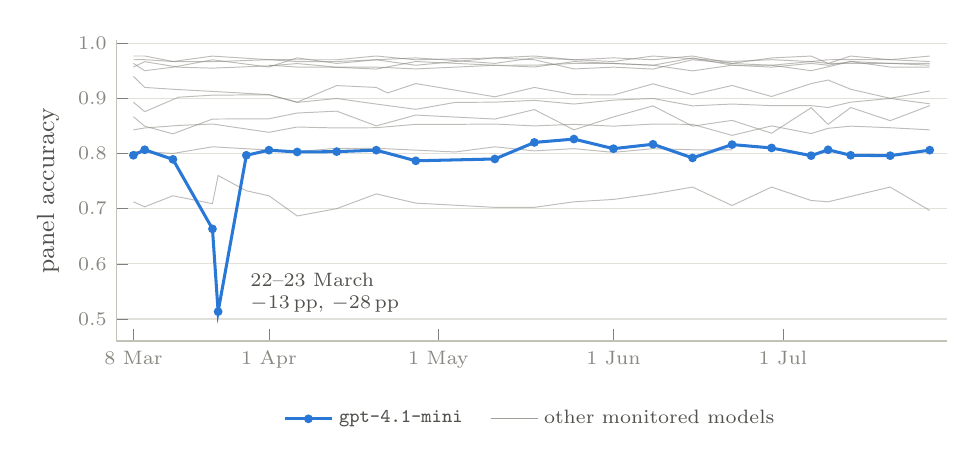
\begin{tikzpicture}
    \begin{axis}[
        width=\linewidth, height=5.4cm,
        xmin=-3, xmax=144, ymin=0.46, ymax=1.005,
        xtick={0,24,54,85,115,146},
        xticklabels={8 Mar,1 Apr,1 May,1 Jun,1 Jul,1 Aug},
        ytick={0.5,0.6,0.7,0.8,0.9,1.0},
        yticklabel style={/pgf/number format/fixed, /pgf/number format/fixed zerofill, /pgf/number format/precision=1},
        ylabel={panel accuracy},
        legend columns=2,
        legend style={at={(0.5,-0.20)}, anchor=north, /tikz/every even column/.append style={column sep=8pt}},
        axis line style={vizaxis, line width=0.4pt},
        tick label style={vizmuted, font=\scriptsize},
        label style={vizink, font=\small},
        legend style={draw=none, fill=none, font=\scriptsize,
                      text=vizink, inner sep=1pt},
        grid=major,
        grid style={vizgrid, line width=0.4pt},
        axis x line*=bottom,
        axis y line*=left,
        ymajorgrids=true,
        xmajorgrids=false,
        clip=false,
    ]
    \addplot[vizmuted, line width=0.35pt, opacity=0.55, forget plot] coordinates {(0,0.8428) (2,0.8462) (8,0.8508) (14,0.8534) (24,0.8383) (29,0.8480) (36,0.8462) (43,0.8467) (50,0.8528) (57,0.8528) (64,0.8533) (71,0.8500) (78,0.8528) (85,0.8495) (92,0.8533) (99,0.8528) (106,0.8328) (113,0.8500) (120,0.8361) (123,0.8456) (127,0.8495) (134,0.8467) (141,0.8428)};
    \addplot[vizmuted, line width=0.35pt, opacity=0.55, forget plot] coordinates {(0,0.8930) (2,0.8758) (8,0.9020) (14,0.9057) (24,0.9064) (29,0.8926) (36,0.8997) (43,0.8896) (50,0.8800) (57,0.8926) (64,0.8930) (71,0.8963) (78,0.8896) (85,0.8967) (92,0.8997) (99,0.8863) (106,0.8896) (113,0.8867) (120,0.8867) (123,0.8833) (127,0.8930) (134,0.8997) (141,0.8900)};
    \addplot[vizmuted, line width=0.35pt, opacity=0.55, forget plot] coordinates {(0,0.9567) (2,0.9664) (8,0.9564) (14,0.9547) (24,0.9588) (29,0.9630) (36,0.9565) (43,0.9565) (50,0.9533) (57,0.9565) (64,0.9599) (71,0.9567) (78,0.9666) (85,0.9632) (92,0.9600) (99,0.9497) (106,0.9599) (113,0.9599) (120,0.9666) (123,0.9632) (127,0.9632) (134,0.9633) (141,0.9600)};
    \addplot[vizmuted, line width=0.35pt, opacity=0.55, forget plot] coordinates {(0,0.8033) (2,0.8033) (7,0.8000) (14,0.8121) (29,0.8033) (36,0.8094) (43,0.8094) (57,0.8027) (64,0.8121) (71,0.8047) (78,0.8087) (85,0.8020) (92,0.8087) (99,0.8067) (106,0.8067)};
    \addplot[vizmuted, line width=0.35pt, opacity=0.55, forget plot] coordinates {(0,0.7124) (2,0.7033) (7,0.7233) (14,0.7090) (15,0.7600) (20,0.7324) (24,0.7233) (29,0.6867) (36,0.7000) (43,0.7267) (50,0.7100) (64,0.7023) (71,0.7023) (78,0.7124) (85,0.7167) (92,0.7267) (99,0.7391) (106,0.7057) (113,0.7391) (120,0.7148) (123,0.7124) (134,0.7391) (141,0.6967)};
    \addplot[vizmuted, line width=0.35pt, opacity=0.55, forget plot] coordinates {(0,0.9699) (2,0.9700) (7,0.9667) (14,0.9765) (24,0.9700) (29,0.9666) (36,0.9667) (43,0.9699) (50,0.9733) (64,0.9633) (71,0.9733) (78,0.9698) (85,0.9733) (92,0.9699) (99,0.9767) (106,0.9633) (113,0.9732) (120,0.9766) (123,0.9632) (127,0.9766) (134,0.9700) (141,0.9766)};
    \addplot[vizmuted, line width=0.35pt, opacity=0.55, forget plot] coordinates {(0,0.9398) (2,0.9197) (7,0.9164) (14,0.9125) (24,0.9067) (29,0.8930) (36,0.9231) (43,0.9197) (45,0.9097) (50,0.9267) (64,0.9027) (71,0.9197) (78,0.9067) (85,0.9060) (92,0.9262) (99,0.9067) (106,0.9233) (113,0.9033) (120,0.9267) (123,0.9331) (127,0.9164) (134,0.9000) (141,0.9133)};
    \addplot[vizmuted, line width=0.35pt, opacity=0.55, forget plot] coordinates {(0,0.8667) (2,0.8495) (7,0.8356) (14,0.8624) (24,0.8629) (29,0.8733) (36,0.8767) (43,0.8500) (50,0.8696) (64,0.8624) (71,0.8796) (78,0.8428) (85,0.8662) (92,0.8863) (99,0.8495) (106,0.8600) (113,0.8367) (120,0.8829) (123,0.8528) (127,0.8833) (134,0.8595) (141,0.8867)};
    \addplot[vizmuted, line width=0.35pt, opacity=0.55, forget plot] coordinates {(0,0.9633) (2,0.9500) (7,0.9564) (14,0.9698) (24,0.9567) (29,0.9733) (36,0.9632) (43,0.9698) (50,0.9599) (64,0.9733) (71,0.9699) (78,0.9532) (85,0.9565) (92,0.9530) (99,0.9699) (106,0.9631) (113,0.9600) (120,0.9500) (127,0.9666) (134,0.9567) (141,0.9564)};
    \addplot[vizmuted, line width=0.35pt, opacity=0.55, forget plot] coordinates {(0,0.9767) (2,0.9767) (7,0.9667) (14,0.9663) (24,0.9700) (29,0.9699) (36,0.9699) (43,0.9767) (50,0.9698) (64,0.9732) (71,0.9767) (78,0.9699) (85,0.9667) (92,0.9767) (106,0.9667) (113,0.9700) (120,0.9666) (123,0.9699) (127,0.9700) (134,0.9700) (141,0.9667)};
    \addplot[vizmuted, line width=0.35pt, opacity=0.55, forget plot] coordinates {(24,0.9600) (29,0.9567) (36,0.9562) (43,0.9530) (50,0.9667) (64,0.9599) (71,0.9600) (78,0.9632) (85,0.9632) (92,0.9599) (99,0.9732) (106,0.9600) (113,0.9565) (120,0.9633) (123,0.9599) (127,0.9667) (134,0.9633) (141,0.9633)};
    \addplot[vizblue, line width=1.1pt, mark=*, mark size=1.0pt, mark options={fill=vizblue, draw=vizblue}] coordinates {(0,0.7967) (2,0.8067) (7,0.7893) (14,0.6633) (15,0.5133) (20,0.7967) (24,0.8060) (29,0.8027) (36,0.8033) (43,0.8060) (50,0.7867) (64,0.7900) (71,0.8200) (78,0.8261) (85,0.8087) (92,0.8167) (99,0.7919) (106,0.8161) (113,0.8100) (120,0.7960) (123,0.8067) (127,0.7967) (134,0.7960) (141,0.8060)};
    \addlegendentry{\texttt{gpt-4.1-mini}}
    \addlegendimage{vizmuted, line width=0.35pt, opacity=0.8}
    \addlegendentry{other monitored models}
    \node[anchor=west, font=\scriptsize, text=vizink, align=left] at (axis cs:19,0.548) {22--23 March\\$-13$\,pp, $-28$\,pp};
    \end{axis}
\end{tikzpicture}
